\documentclass[border=8pt]{standalone}
\usepackage{tikz}
\usetikzlibrary{decorations.pathreplacing}
\begin{document}
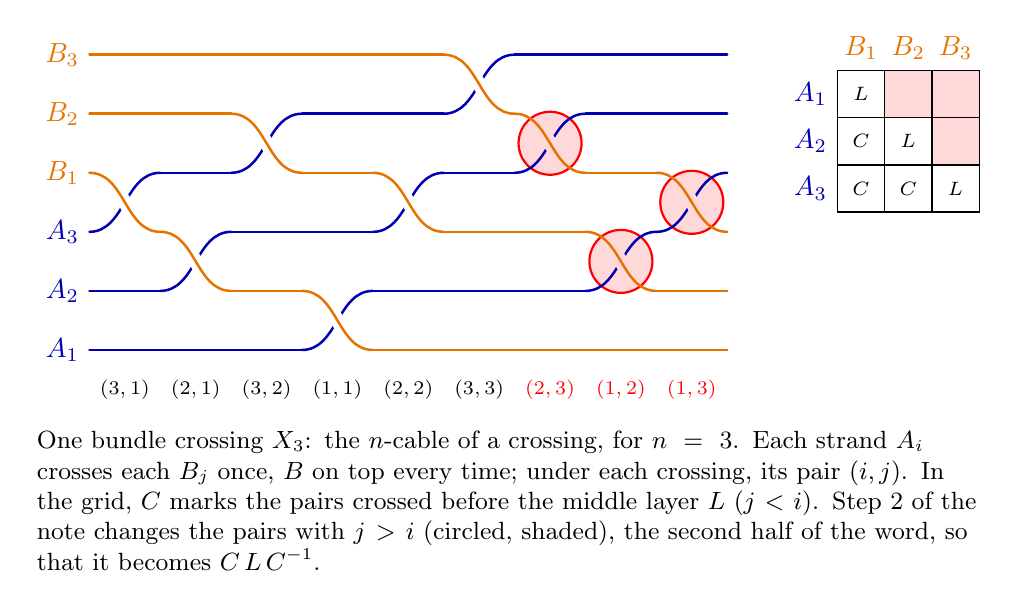
\begin{tikzpicture}[line width=0.9pt, line cap=round]
\draw[blue!70!black] (0.000,0.000) -- (0.900,0.000);
\draw[blue!70!black] (0.000,0.750) -- (0.900,0.750);
\draw[orange!90!black] (0.000,3.000) -- (0.900,3.000);
\draw[orange!90!black] (0.000,3.750) -- (0.900,3.750);
\draw[blue!70!black] (0.000,1.500) .. controls (0.450,1.500) and (0.450,2.250) .. (0.900,2.250);
\begin{scope}\clip (0.450,1.875) circle (0.3);\draw[white, line width=5pt] (0.000,2.250) .. controls (0.450,2.250) and (0.450,1.500) .. (0.900,1.500);\end{scope}
\draw[orange!90!black] (0.000,2.250) .. controls (0.450,2.250) and (0.450,1.500) .. (0.900,1.500);
\draw[blue!70!black] (0.900,0.000) -- (1.800,0.000);
\draw[blue!70!black] (0.900,2.250) -- (1.800,2.250);
\draw[orange!90!black] (0.900,3.000) -- (1.800,3.000);
\draw[orange!90!black] (0.900,3.750) -- (1.800,3.750);
\draw[blue!70!black] (0.900,0.750) .. controls (1.350,0.750) and (1.350,1.500) .. (1.800,1.500);
\begin{scope}\clip (1.350,1.125) circle (0.3);\draw[white, line width=5pt] (0.900,1.500) .. controls (1.350,1.500) and (1.350,0.750) .. (1.800,0.750);\end{scope}
\draw[orange!90!black] (0.900,1.500) .. controls (1.350,1.500) and (1.350,0.750) .. (1.800,0.750);
\draw[blue!70!black] (1.800,0.000) -- (2.700,0.000);
\draw[orange!90!black] (1.800,0.750) -- (2.700,0.750);
\draw[blue!70!black] (1.800,1.500) -- (2.700,1.500);
\draw[orange!90!black] (1.800,3.750) -- (2.700,3.750);
\draw[blue!70!black] (1.800,2.250) .. controls (2.250,2.250) and (2.250,3.000) .. (2.700,3.000);
\begin{scope}\clip (2.250,2.625) circle (0.3);\draw[white, line width=5pt] (1.800,3.000) .. controls (2.250,3.000) and (2.250,2.250) .. (2.700,2.250);\end{scope}
\draw[orange!90!black] (1.800,3.000) .. controls (2.250,3.000) and (2.250,2.250) .. (2.700,2.250);
\draw[blue!70!black] (2.700,1.500) -- (3.600,1.500);
\draw[orange!90!black] (2.700,2.250) -- (3.600,2.250);
\draw[blue!70!black] (2.700,3.000) -- (3.600,3.000);
\draw[orange!90!black] (2.700,3.750) -- (3.600,3.750);
\draw[blue!70!black] (2.700,0.000) .. controls (3.150,0.000) and (3.150,0.750) .. (3.600,0.750);
\begin{scope}\clip (3.150,0.375) circle (0.3);\draw[white, line width=5pt] (2.700,0.750) .. controls (3.150,0.750) and (3.150,0.000) .. (3.600,0.000);\end{scope}
\draw[orange!90!black] (2.700,0.750) .. controls (3.150,0.750) and (3.150,0.000) .. (3.600,0.000);
\draw[orange!90!black] (3.600,0.000) -- (4.500,0.000);
\draw[blue!70!black] (3.600,0.750) -- (4.500,0.750);
\draw[blue!70!black] (3.600,3.000) -- (4.500,3.000);
\draw[orange!90!black] (3.600,3.750) -- (4.500,3.750);
\draw[blue!70!black] (3.600,1.500) .. controls (4.050,1.500) and (4.050,2.250) .. (4.500,2.250);
\begin{scope}\clip (4.050,1.875) circle (0.3);\draw[white, line width=5pt] (3.600,2.250) .. controls (4.050,2.250) and (4.050,1.500) .. (4.500,1.500);\end{scope}
\draw[orange!90!black] (3.600,2.250) .. controls (4.050,2.250) and (4.050,1.500) .. (4.500,1.500);
\draw[orange!90!black] (4.500,0.000) -- (5.400,0.000);
\draw[blue!70!black] (4.500,0.750) -- (5.400,0.750);
\draw[orange!90!black] (4.500,1.500) -- (5.400,1.500);
\draw[blue!70!black] (4.500,2.250) -- (5.400,2.250);
\draw[blue!70!black] (4.500,3.000) .. controls (4.950,3.000) and (4.950,3.750) .. (5.400,3.750);
\begin{scope}\clip (4.950,3.375) circle (0.3);\draw[white, line width=5pt] (4.500,3.750) .. controls (4.950,3.750) and (4.950,3.000) .. (5.400,3.000);\end{scope}
\draw[orange!90!black] (4.500,3.750) .. controls (4.950,3.750) and (4.950,3.000) .. (5.400,3.000);
\draw[orange!90!black] (5.400,0.000) -- (6.300,0.000);
\draw[blue!70!black] (5.400,0.750) -- (6.300,0.750);
\draw[orange!90!black] (5.400,1.500) -- (6.300,1.500);
\draw[blue!70!black] (5.400,3.750) -- (6.300,3.750);
\fill[red!15] (5.850,2.625) circle (0.4);
\draw[red, thick] (5.850,2.625) circle (0.4);
\draw[blue!70!black] (5.400,2.250) .. controls (5.850,2.250) and (5.850,3.000) .. (6.300,3.000);
\begin{scope}\clip (5.850,2.625) circle (0.3);\draw[red!15, line width=5pt] (5.400,3.000) .. controls (5.850,3.000) and (5.850,2.250) .. (6.300,2.250);\end{scope}
\draw[orange!90!black] (5.400,3.000) .. controls (5.850,3.000) and (5.850,2.250) .. (6.300,2.250);
\draw[orange!90!black] (6.300,0.000) -- (7.200,0.000);
\draw[orange!90!black] (6.300,2.250) -- (7.200,2.250);
\draw[blue!70!black] (6.300,3.000) -- (7.200,3.000);
\draw[blue!70!black] (6.300,3.750) -- (7.200,3.750);
\fill[red!15] (6.750,1.125) circle (0.4);
\draw[red, thick] (6.750,1.125) circle (0.4);
\draw[blue!70!black] (6.300,0.750) .. controls (6.750,0.750) and (6.750,1.500) .. (7.200,1.500);
\begin{scope}\clip (6.750,1.125) circle (0.3);\draw[red!15, line width=5pt] (6.300,1.500) .. controls (6.750,1.500) and (6.750,0.750) .. (7.200,0.750);\end{scope}
\draw[orange!90!black] (6.300,1.500) .. controls (6.750,1.500) and (6.750,0.750) .. (7.200,0.750);
\draw[orange!90!black] (7.200,0.000) -- (8.100,0.000);
\draw[orange!90!black] (7.200,0.750) -- (8.100,0.750);
\draw[blue!70!black] (7.200,3.000) -- (8.100,3.000);
\draw[blue!70!black] (7.200,3.750) -- (8.100,3.750);
\fill[red!15] (7.650,1.875) circle (0.4);
\draw[red, thick] (7.650,1.875) circle (0.4);
\draw[blue!70!black] (7.200,1.500) .. controls (7.650,1.500) and (7.650,2.250) .. (8.100,2.250);
\begin{scope}\clip (7.650,1.875) circle (0.3);\draw[red!15, line width=5pt] (7.200,2.250) .. controls (7.650,2.250) and (7.650,1.500) .. (8.100,1.500);\end{scope}
\draw[orange!90!black] (7.200,2.250) .. controls (7.650,2.250) and (7.650,1.500) .. (8.100,1.500);
\node[left, blue!70!black] at (0,0.000) {$A_1$};
\node[left, blue!70!black] at (0,0.750) {$A_2$};
\node[left, blue!70!black] at (0,1.500) {$A_3$};
\node[left, orange!90!black] at (0,2.250) {$B_1$};
\node[left, orange!90!black] at (0,3.000) {$B_2$};
\node[left, orange!90!black] at (0,3.750) {$B_3$};
\node[black, font=\scriptsize] at (0.450,-0.500) {$(3,1)$};
\node[black, font=\scriptsize] at (1.350,-0.500) {$(2,1)$};
\node[black, font=\scriptsize] at (2.250,-0.500) {$(3,2)$};
\node[black, font=\scriptsize] at (3.150,-0.500) {$(1,1)$};
\node[black, font=\scriptsize] at (4.050,-0.500) {$(2,2)$};
\node[black, font=\scriptsize] at (4.950,-0.500) {$(3,3)$};
\node[red, font=\scriptsize] at (5.850,-0.500) {$(2,3)$};
\node[red, font=\scriptsize] at (6.750,-0.500) {$(1,2)$};
\node[red, font=\scriptsize] at (7.650,-0.500) {$(1,3)$};
\node[blue!70!black, left] at (9.50,3.25) {$A_1$};
\draw[fill=white, line width=0.5pt] (9.50,2.95) rectangle (10.10,3.55);
\node[font=\scriptsize] at (9.80,3.25) {$L$};
\draw[fill=red!15, line width=0.5pt] (10.10,2.95) rectangle (10.70,3.55);
\draw[fill=red!15, line width=0.5pt] (10.70,2.95) rectangle (11.30,3.55);
\node[blue!70!black, left] at (9.50,2.65) {$A_2$};
\draw[fill=white, line width=0.5pt] (9.50,2.35) rectangle (10.10,2.95);
\node[font=\scriptsize] at (9.80,2.65) {$C$};
\draw[fill=white, line width=0.5pt] (10.10,2.35) rectangle (10.70,2.95);
\node[font=\scriptsize] at (10.40,2.65) {$L$};
\draw[fill=red!15, line width=0.5pt] (10.70,2.35) rectangle (11.30,2.95);
\node[blue!70!black, left] at (9.50,2.05) {$A_3$};
\draw[fill=white, line width=0.5pt] (9.50,1.75) rectangle (10.10,2.35);
\node[font=\scriptsize] at (9.80,2.05) {$C$};
\draw[fill=white, line width=0.5pt] (10.10,1.75) rectangle (10.70,2.35);
\node[font=\scriptsize] at (10.40,2.05) {$C$};
\draw[fill=white, line width=0.5pt] (10.70,1.75) rectangle (11.30,2.35);
\node[font=\scriptsize] at (11.00,2.05) {$L$};
\node[orange!90!black, above] at (9.80,3.55) {$B_1$};
\node[orange!90!black, above] at (10.40,3.55) {$B_2$};
\node[orange!90!black, above] at (11.00,3.55) {$B_3$};
\node[anchor=north west, text width=12.10cm, font=\small] at (-0.80,-0.90) {One bundle crossing $X_3$: the $n$-cable of a crossing, for $n = 3$. Each strand $A_i$ crosses each $B_j$ once, $B$ on top every time; under each crossing, its pair $(i,j)$. In the grid, $C$ marks the pairs crossed before the middle layer $L$ ($j < i$). Step 2 of the note changes the pairs with $j > i$ (circled, shaded), the second half of the word, so that it becomes $C\,L\,C^{-1}$.};
\end{tikzpicture}
\end{document}
